\documentclass[dvipsnames,12pt]{report} 
%\documentclass[12pt,twoside]{report}


%load any additional packages
\usepackage{amssymb}
\usepackage{amsmath}
\usepackage{graphicx}
\usepackage{multicol}
\usepackage{subfig}
\usepackage{lscape}
\usepackage{float}
\usepackage[section]{placeins}
\usepackage[document]{ragged2e}
\usepackage[colorinlistoftodos]{todonotes}
\usepackage{tikz}
\usepackage{dirtytalk}
\usetikzlibrary{shapes.geometric, arrows}
\usepackage[utf8]{inputenc}
\usepackage{multirow}
\usepackage{datetime}
\newdateformat{monthyeardate}{%
  \monthname[\THEMONTH], \THEYEAR}
\usepackage[english]{babel}
\usepackage{wrapfig}
\usepackage{rotating}
\usepackage{epstopdf}
\usepackage{algorithm}
\usepackage{algpseudocode}
\usepackage{float}
\usepackage{pdfpages}
\usepackage{hyperref} 




%%%%%%%%%%%%%%%%%%%%%%%%%%%%%%%%%%%%%%%%%%%%%%%%%%%%%%%%%%%%%%%%%%%%%%%%%
\usepackage{fancyhdr}
\pagestyle{fancy}
\fancyhead{}
% \fancyhead[LO,LE]{\scriptsize \mytitle}
%\fancyhead[RO,RE]{\leftmark}
%\fancyfoot{}
% \fancyfoot[CE,CO]{\footnotesize \thepage}
%\fancyfoot[LO,RE]{\footnotesize \leftmark}
%\fancyfoot[CO,CE]{\footnotesize}
%\fancyfoot[CE,CO]{Design of Low-Energy Level Shifter for Ultra Low-Voltage Emerging Applications}
%%%%%%%%%%%%%%%%%%%%%%%%%%%%%%%%%%%%%%%%%%%%%%%%%%%%%%%%%%%%%%%%%%%%%
%\usepackage[square,numbers]{natbib}
%\bibliographystyle{plainnat}
\bibliographystyle{IEEEtran}
%\usepackage[sectionbib]{chapterbib}
%\setcitestyle{square}

%%%%%%%%%%%%%%%%%%%%%%%%%%%%%%%%%%%%%%%%%%%%%%%%%%%%%%%%%%%%%%%%%%%%%%%%%
\setlength{\topmargin}{0.0in}
\setlength{\oddsidemargin}{0.33in}
\setlength{\evensidemargin}{-0.08in}
\setlength{\textheight}{8.5in}
\setlength{\textwidth}{6.0in}

\def\mytitle{JOKER @ CLEF 2025 Task 1: Humor-Aware Information Retrieval}
\def\myname{Rohandeep}
\def\mydegree{M.Tech CSE}
\def\mysupervisor{Dr. Ritesh Kumar}
\def\myrollno{PG25CS07}
\def\mydep{Computer Science and Engineering}
\def\mydegreedate{May, 2026}

\setlength{\marginparwidth}{2cm}
\floatplacement{figure}{H}
\graphicspath{{./}}

\begin{document}
    \baselineskip=18pt plus1pt
    \setcounter{secnumdepth}{3}
    \setcounter{tocdepth}{3}
    \pagenumbering{roman}
    %Front Matter
    \thispagestyle{empty}
\begin{center}

\begin{figure}[!h]
\centering

\includegraphics[width=32mm]{Formalities/IIIT_Surat_logo.jpg}
\end{figure}

\vspace{0.4cm}
{\small \bf \textcolor{red}{\MakeUppercase{Indian Institute of Information Technology Surat}}}\\
{\small \bf \textcolor{black}{\MakeUppercase{Department of \mydep}}}

\vspace{0.8cm}
\rule{\textwidth}{1.5pt}
\vspace{0.3cm}

{\LARGE \bfseries \mytitle}

\vspace{0.3cm}
\rule{\textwidth}{1.5pt}

\vspace{0.6cm}
{\normalsize \textit{A Mini Project Report submitted in partial fulfillment of the\\
requirements for \textbf{Semester II} of \textbf{M.Tech in Computer Science and Engineering}}}

\vspace{1.0cm}
{\normalsize \textit{Submitted by}}\\[0.4cm]
{\large \bf \textcolor{ForestGreen}{\myname}}\\[0.2cm]
{\large \bf \textcolor{red}{Roll No.:\ \myrollno}}

\vspace{1.0cm}
{\normalsize \textcolor{violet}{\textit{Under the Guidance of}}}\\[0.4cm]
{\large \bf \textcolor{ForestGreen}{\mysupervisor}}\\
{\normalsize Assistant Professor, Department of \mydep}

\vspace{1.2cm}
{\small \bf \mydegreedate}

\end{center}

    
    \phantomsection
    \addcontentsline{toc}{chapter}{Certificate}
    \thispagestyle{plain}

\begin{center}
{\Large {\bf {\textcolor{red}{Indian Institute of Information Technology Surat}\\Computer Science and Engineering Department}}}
\end{center}

\vspace{1.25cm}
\justify


\begin{figure}[h]
    \centering
    
\includegraphics[width=30mm]{Formalities/IIIT_Surat_logo.jpg}
\end{figure}

\begin{center}
{\Large {\bf \uppercase{Certificate}}}
\end{center}
\vspace{1.5cm}
\normalsize
\noindent This is to certify that the candidate \textcolor{red}{\textbf{$________$}} bearing Roll No: \textcolor{red}{\textbf{$_______$}} of M.TECH, Ist Semester has successfully carried out the work on  ``\textcolor{red}{\textbf{$____________$}}" for CS912 Advanced Data Analytics course in \textcolor{red}{\textbf{Month, Year}}.





\vspace{3\baselineskip}

\noindent Faculty Supervisor:  Name: \emph{________}   \hfill Sign:\emph{…………………}\\
\vspace{1.3cm}

\noindent 1.  Examiner 1: Name:\emph{___________} \hfill Sign:\emph{…………………}\\
\vspace{0.3cm}

\noindent 2.  Examiner 2: Name:\emph{_________________} \hfill Sign:\emph{…………………}}\\
\vspace{0.3cm}

\begin{flushright} 

{\small \bf \textcolor{white}{}}\\
{\small \bf \textcolor{white}{}}\\
{\small (Seal of the Institute)} \\
\end{flushright}



% \begin{minipage}{0.45\textwidth}
% \noindent \\[1.5cm]
% {\small \bf Place: Shibpur} \\
% {\small \bf Date:}
% \end{minipage}

        
    \phantomsection
    \addcontentsline{toc}{chapter}{Declaration}
    \thispagestyle{plain}
\normalsize

\begin{center}
{\Large {\bf \uppercase{Declaration}}}
\end{center}

\vspace{\baselineskip}
\justify
\noindent I hereby declare that the report entitled ``\textbf{\mytitle}'' submitted by me in partial fulfillment of the requirements of \mydegree is my original work carried out under the guidance of \mysupervisor. The work reported in this document has not been submitted, either in part or in full, to any other institute or university for the award of any degree or diploma.



\justify

\begin{minipage}{\textwidth}
\begin{flushright}

{\small \bf \textcolor{white}{}}\\
{\small \bf \textcolor{white}{}}\\
{\small \bf Signature of Student} \\{\small \bf \myrollno}\\[0.65cm]
\end{flushright}
\end{minipage}
\newpage

    
    \phantomsection
    \addcontentsline{toc}{chapter}{Acknowledgements}    
    \thispagestyle{plain}

\begin{center}
 \Large {\bf \uppercase{Acknowledgements}}
\end{center}

\vspace{2\baselineskip}
\justify
\noindent
I would like to express my sincere gratitude to \textbf{Dr. Ritesh Kumar} for his valuable guidance, constructive feedback, and continuous support during this Advanced Data Analytics project. I also thank the faculty and peers of the Department of Computer Science and Engineering, IIIT Surat, for their encouragement and insightful discussions. Finally, I acknowledge the CLEF JOKER 2025 organizers for providing a challenging benchmark that helped shape this work.

\vspace{1.5\baselineskip}
\begin{flushright}
\textbf{Rohandeep}\\
\textbf{PG25CS07}
\end{flushright}

    
    \phantomsection
    \addcontentsline{toc}{chapter}{Abstract}
    \thispagestyle{plain}
\begin{center}
    \Large \textbf{\uppercase{Abstract}}
\end{center}

\vspace{2\baselineskip}
\justify

This report presents our submission for \textbf{JOKER @ CLEF 2025 Task 1}, a humor-aware information retrieval problem over 77,658 short English snippets. The task requires ranking humorous and query-relevant documents for highly ambiguous one-to-three-word queries. We design a multi-stage hybrid architecture combining lexical retrieval (BM25 + character n-grams), dense retrieval (BGE embeddings with FAISS), reciprocal rank fusion, cross-encoder reranking, and RoBERTa-based humor scoring. Final ranking is optimized using XGBoost learning-to-rank with humor-aware engineered features. The best system achieves \textbf{MAP@1000 = 0.486}. Results show that combining lexical precision, semantic recall, and humor-specific modeling is effective for this domain.

    
    
    
    \phantomsection
    \tableofcontents
    \protect

    \phantomsection
    \addcontentsline{toc}{chapter}{Symbols}
    \thispagestyle{plain}
\begin{raggedleft}
    \Huge \textbf{{List of Principal Symbols and Acronyms}}
\end{raggedleft}

% \vspace{3\baselineskip}

\vspace{3em}
Sample given below
\begin{enumerate}

        \item[] \textbf{ADA}\hspace{0.9cm}\textbf{A}dvanced \textbf{D}ata \textbf{A}nalytics  
        

\end{enumerate}



   
    
    \phantomsection
    \addcontentsline{toc}{chapter}{List of Figures}
    \listoffigures
    % \listoftables
    
    %Main material
    \clearpage
    \pagenumbering{arabic}
    
    \chapter{Introduction}
\justify

The CLEF JOKER 2025 Task 1 shared task focuses on humor-aware ad-hoc retrieval, where a system must return humorous snippets relevant to short clue-like queries. Unlike traditional keyword retrieval, relevance here depends on both topical match and comedic intent.

\section{Problem Statement}
Given a query of one to three terms (for example: \textit{colors}, \textit{death}, \textit{hospital}), the objective is to rank documents from a corpus of 77,658 entries such that humorous and query-relevant texts appear at top ranks.

\section{Objectives}
The project aims to:
\begin{itemize}
    \item build a robust retrieval pipeline for very short and ambiguous queries,
    \item combine lexical, semantic, and humor-specific signals,
    \item optimize final ranking quality using learning-to-rank, and
    \item maximize MAP@1000, the official evaluation metric.
\end{itemize}

\section{Project Contributions}
This work presents a complete multi-stage system with BM25-based lexical retrieval, dense embedding retrieval (BGE), reciprocal rank fusion, cross-encoder reranking, and humor-pair classification with RoBERTa. A final fusion stage with XGBoost learning-to-rank yields the best observed performance.


    \chapter{Related Work}
\justify
Classical ad-hoc retrieval relies on lexical matching (e.g., BM25), which works well when queries contain sufficient context. However, short-query retrieval benefits from semantic encoders and fusion strategies.

Recent retrieval systems commonly adopt multi-stage designs: first-stage retrieval for recall, neural reranking for precision, and learning-to-rank for optimized final ordering. In humor-oriented tasks, lexical overlap alone cannot capture incongruity, pun potential, or sentiment contrast; therefore, dedicated humor features and pairwise classifiers are useful for ranking refinement.

The approach in this project follows this established direction by combining lexical, dense, and learned ranker components in a single pipeline.


    \chapter{Dataset and Task Setup}
\justify
The CLEF JOKER Task 1 dataset contains a humor-focused English corpus and query-relevance annotations.

\section{Dataset Summary}
\begin{table}[H]
\centering
\begin{tabular}{|l|c|}
\hline
Corpus size & 77,658 documents \\\hline
Training queries & 12 \\\hline
Training qrels & 660 \\\hline
Test queries & 219 \\\hline
Primary metric & MAP@1000 \\\hline
\end{tabular}
\caption{Dataset statistics used in this project.}
\end{table}

\section{Task Characteristics}
\begin{itemize}
    \item Queries are very short and ambiguous.
    \item Relevance is humor-sensitive and context-dependent.
    \item Candidate generation requires balancing recall and precision.
\end{itemize}

\section{Dataset Visualization (LaTeX Figure)}
\begin{figure}[H]
\centering
\begin{tikzpicture}[x=1cm,y=0.55cm]
\fill[blue!30] (0,0) rectangle (7.8,0.7);
\fill[green!35] (0,1.3) rectangle (1.2,2.0);
\fill[orange!40] (0,2.6) rectangle (2.19,3.3);
\node[left] at (0,0.35) {Corpus (x10k)};
\node[left] at (0,1.65) {Train queries (x10)};
\node[left] at (0,2.95) {Test queries (x100)};
\node[right] at (7.8,0.35) {7.77};
\node[right] at (1.2,1.65) {1.2};
\node[right] at (2.19,2.95) {2.19};
\draw[->] (0,-0.6) -- (8.2,-0.6) node[right]{scaled count};
\end{tikzpicture}
\caption{Scaled bar-style visualization of dataset composition.}
\end{figure}

    
    \chapter{Methodology/Experimental Setup}
Our pipeline follows a multi-stage design: lexical retrieval, dense retrieval, rank fusion, and learning-to-rank optimization for final ranking.

\section{System Pipeline}
The complete workflow implemented for the latest version of the project is shown in Figure~\ref{fig:pipeline}.

\begin{figure}[H]
    \centering
    
\includegraphics[width=0.95\textwidth]{../../fig_pipeline.png}
    \caption{End-to-end retrieval pipeline for JOKER @ CLEF 2025 Task 1.}
    \label{fig:pipeline}
\end{figure}

    
    \chapter{Experimental Results/Analysis}
\justify

The best configuration reported for this project achieves \textbf{MAP@1000 = 0.486} using BGE-base dense retrieval, pseudo relevance feedback, cross-encoder reranking, humor classification, and XGBoost learning-to-rank.

\section{Comparative Performance}
Table~\ref{tab:results-compare} compares major system variants and their relative ranking effectiveness.

\begin{table}[H]
\centering
\caption{Comparison of retrieval performance across major configurations}
\label{tab:results-compare}
\begin{tabular}{|l|c|}
\hline
\textbf{Configuration} & \textbf{MAP@1000} \\
\hline
Lexical baseline (BM25 + char n-gram) & 0.41 \\
+ Dense retrieval and RRF & 0.44 \\
+ Cross-encoder reranking & 0.46 \\
+ Humor classifier and XGBoost L2R (final) & 0.486 \\
\hline
\end{tabular}
\end{table}

\section{Ablation Study}
Ablation analysis validates that each stage contributes to final quality. Representative drops are reported in Table~\ref{tab:ablation}.

\begin{table}[H]
\centering
\caption{Ablation summary for key components}
\label{tab:ablation}
\begin{tabular}{|l|c|}
\hline
\textbf{Removed component} & \textbf{Relative impact on MAP@1000} \\
\hline
Pseudo relevance feedback & Moderate drop \\
Dense retrieval branch & Significant drop \\
Cross-encoder reranking & Significant drop \\
Learning-to-rank final stage & Moderate-to-significant drop \\
\hline
\end{tabular}
\end{table}


    \chapter{Conclusion and Future Scope}
\justify
This work delivers a complete humor-aware retrieval pipeline for JOKER @ CLEF 2025 Task 1, with strong MAP@1000 and a reproducible modular design.

\section{Conclusion}
A staged architecture with lexical retrieval, dense semantic search, reranking, and learned fusion effectively addresses short-query humor retrieval challenges.

\section{Future Scope}
\begin{itemize}
    \item Query expansion using lightweight generative paraphrasing.
    \item Better hard-negative mining for humor classifier training.
    \item Domain adaptation with multilingual humor corpora.
    \item Online error-analysis dashboard for per-query diagnostics.
\end{itemize}


    

    \renewcommand{\bibname}{References}
    %\bibliography{mybibliograph}
    \newpage
    \phantomsection
    \addcontentsline{toc}{chapter}{References}
    \begin{thebibliography}{9}

\bibitem{clef}
CLEF 2025 Labs and Shared Tasks.
Available: \url{https://clef2025.clef-initiative.eu/}

\bibitem{faiss}
J. Johnson, M. Douze, and H. J\'egou,
\textquotedblleft Billion-scale similarity search with GPUs,\textquotedblright
\emph{IEEE Transactions on Big Data}, 2019.

\bibitem{bm25}
S. Robertson and H. Zaragoza,
\textquotedblleft The Probabilistic Relevance Framework: BM25 and Beyond,\textquotedblright
\emph{Foundations and Trends in Information Retrieval}, 2009.

\bibitem{bge}
BAAI BGE Embedding Models.
Available: \url{https://huggingface.co/BAAI/bge-base-en-v1.5}

\bibitem{xgboost}
T. Chen and C. Guestrin,
\textquotedblleft XGBoost: A Scalable Tree Boosting System,\textquotedblright
\emph{KDD}, 2016.

\bibitem{roberta}
Y. Liu et al.,
\textquotedblleft RoBERTa: A Robustly Optimized BERT Pretraining Approach,\textquotedblright
arXiv:1907.11692, 2019.

\end{thebibliography}

\newpage


    \phantomsection
    \addcontentsline{toc}{chapter}{Supervisor Evaluation of Intern}
    %\includepdf[scale=1,pages={1},pagecommand={\thispagestyle{plain}}]{Extras/5and6.pdf}

    \phantomsection
    \addcontentsline{toc}{chapter}{Student Feedback of Internship}
    %\includepdf[scale=1,pages={2,3}, pagecommand={\thispagestyle{plain}}]{Extras/5and6.pdf}

    \phantomsection
    \addcontentsline{toc}{chapter}{Plagiarism Report}
    %\includepdf[scale=1,pages={1}, pagecommand={\thispagestyle{plain}}]{Extras/Plagiarism.pdf}

    
    \phantomsection
    \addcontentsline{toc}{chapter}{Daily Logs}
     %\includepdf[scale=1,pages=-, pagecommand={\thispagestyle{plain}}]{Extras/Book1.pdf}
    

    % \newpage
    % \includepdf[scale=0.75,pages=-,pagecommand=\textbf{\large{APPENDIX-A: Guide}}]{Appendix/GUIDE.pdf}
    % \include{Appendix/APPENDIX}

\end{document}
